\chapter{Simulation}\label{chap:Simulation}

This chapter presents simulation results obtained on the system presented in \cref{chap:WDN} and will cover both Tabular Q-learning and function approximation Q-learning. Each section begins with a hyperparameter search using a sweep, followed by the simulation results using those parameters. Approximation is first done only on height, then also on time.

All simulation results obtained use the barrier function presented in \cref{sec:CostFuncAndState-ActionSelection} with left and right side zeros at 20 and 40 respectively. The height discretisation is done according to \cref{eq:HeightStates}, with $h_{lower} = 15$ and $h_{upper} = 55$. Time is discretised into 24 states, one for each hour in a day. $Q$ and $\textbf{w}$ are initialised to 0.

Most of simulations are done where the last 10$\%$ of iterations are without learning or randomness, we will refer to this area as the cutoff. This gives a more explicit indication of performance\footnote{E.g. a large epsilon can result in higher cost while learning, but lower cost \textit{after learning}, this behaviour is hidden without the \textit{cutoff}}.

Note we have setup the simulation to match laboratory values, but time scales are not similar.

\newpage \clearpage


\section{Tabular Q-learning}\label{sec:SimTabularQ}

The following section presents results obtained when applying tabular Q-learning to the water distribution nentwork presented in \cref{chap:WDN}. Action values are updated according to \cref{alg:Q-learning}.

\subsection{Hyperparameter Sweep}\label{sec:TabularHSweep}
Sweeps are performed over singular parameters, ideally combinations of all parameters should be swept, but we deem this too resource demanding. Performance is evaluated by looking at a moving average of the cost with a large window size, a large window smooths out randomness and clears up tendencies. The moving average is calculated by finding the mean of neighbouring elements from a point, a window size of 5760 is used determining how many neighbouring points are included. In the beginning and end where there are not enough neighbouring points to fill the window, it is truncated to include as many neighbouring points as possible.

Sequential sweeps over single parameters are bound to have some iterative nature going back and forth. Initial values are found by doing a fast and coarse sweep of all parameters to find suitable values, these initial sweeps are not shown here as they receive no further thought than to get started.

Initial values are shown below in the order they are swept:

\begin{equation*}
	\alpha = 0.5 \hspace{1cm} \gamma = 0.9 \hspace{1cm} \epsilon = 0.1
\end{equation*}

\begin{figure}[h!]
	\centering
	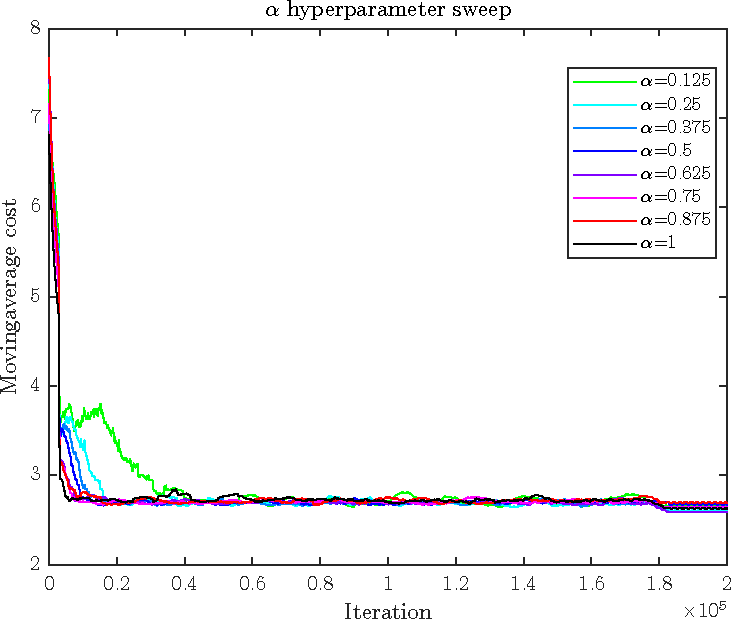
\includegraphics[width=0.7\linewidth]{figures/AlphaSweepTabRealHFull.pdf}
	\caption{Alpha sweep using 200000 iterations.}
	\label{fig:AlphaSweepTabularFull}
\end{figure} 

\begin{figure}
	\centering
	\begin{subfigure}{.5\textwidth}
		\centering
		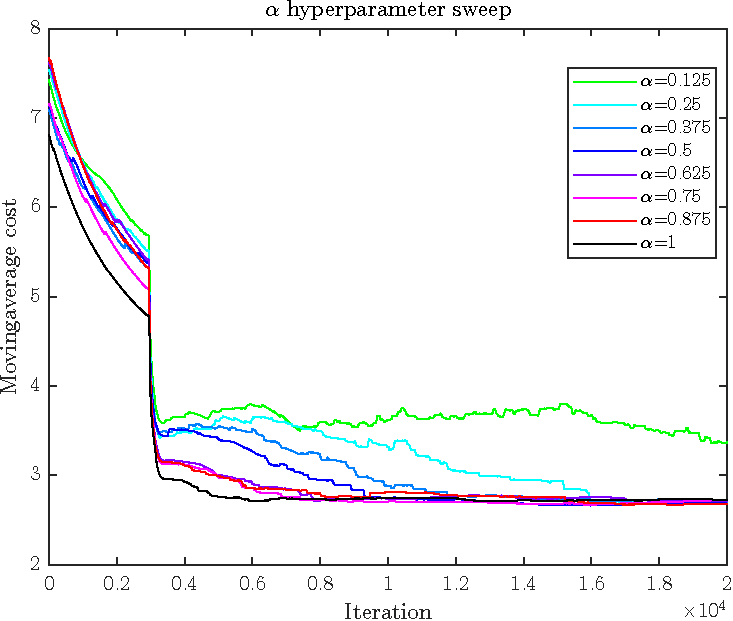
\includegraphics[width=1\linewidth]{figures/AlphaSweepTabRealHLeft.pdf}
		\caption{Initial convergence.}
		\label{fig:AlphaSweepTabularLeft}
	\end{subfigure}%
	\begin{subfigure}{.5\textwidth}
		\centering
		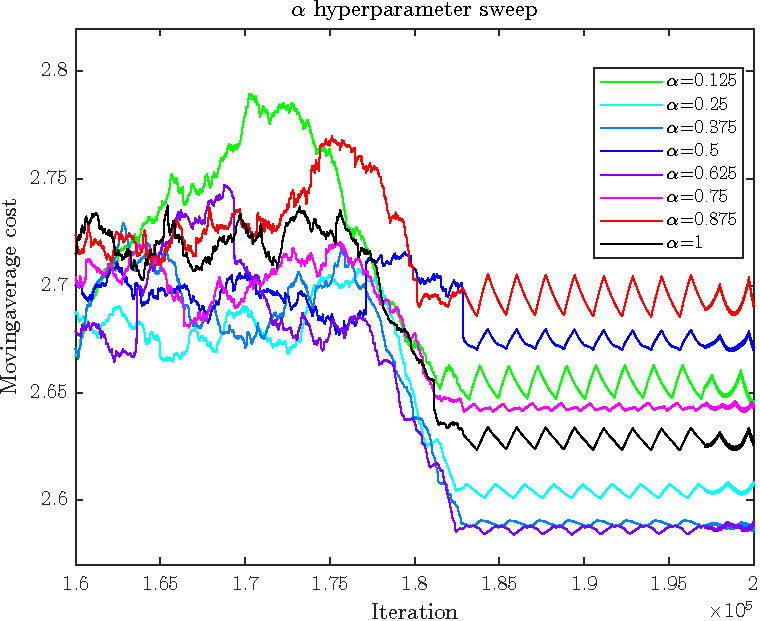
\includegraphics[width=1\linewidth]{figures/AlphaSweepTabRealHRight.pdf}
		\caption{Cutoff convergence.}
		\label{fig:AlphaSweepTabularRight}
	\end{subfigure}
	\caption{Zoomed images of left and right side of \cref{fig:AlphaSweepTabularFull} focusing on initial convergence and cutoff convergence.}
	\label{fig:Leftandright}
\end{figure}

\cref{fig:AlphaSweepTabularFull} shows how the moving average at different $\alpha$ values converge, see \cref{fig:Leftandright} for zoomed plots of beginning and end of the sweep. The long middle section for which it looks like all values have settled, is included to see if some values ultimately converge to a lower cost if it is allowed to see many random actions. The only clear tendency is that higher values converge faster.
In the final 10$\%$, no values appear better within the margin of randomness. Higher values are more susceptible to the random actions performed leading up to the cutoff, meaning there is a slightly larger spread of their final convergence cost.

\begin{figure}
	\centering
	\begin{subfigure}{.5\textwidth}
		\centering
		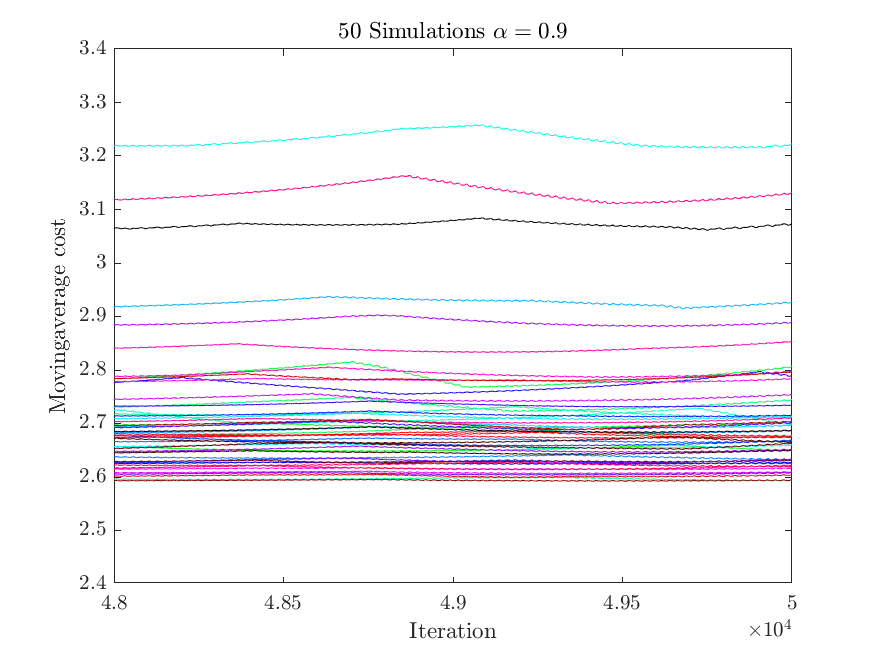
\includegraphics[width=1\linewidth]{figures/50plot09.pdf}
		\caption{Cutoff convergence of 50 simulations using $\alpha = 0.9$.}
		\label{fig:50plot09}
	\end{subfigure}%
	\begin{subfigure}{.5\textwidth}
		\centering
		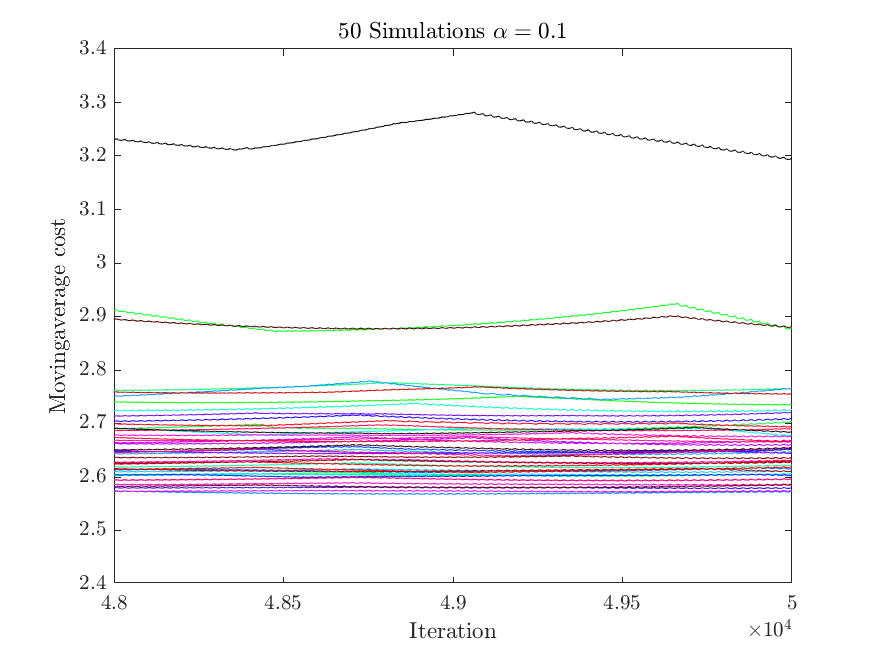
\includegraphics[width=1\linewidth]{figures/50plot01.pdf}
		\caption{Cutoff convergence of 50 simulations using $\alpha = 0.1$.}
		\label{fig:50plot01}
	\end{subfigure}
	\caption{Comparison of cutoff convergence of 50 simulations using $\alpha = 0.9$ and $\alpha = 0.1$. Notice colours do not carry meaning, as Matlab cannot distinguish 50 plots with different colours.}
	\label{fig:50plot}
\end{figure}

This tendency has been further explored by simulating values of $\alpha = 0,1$ and $\alpha = 0.9$ 50 times for 50000 iterations, see \cref{fig:50plot}. Higher values clearly show a higher variance. We also think the wider spread is due to higher $\alpha$ values \textit{bouncing} around the optimal minimum of the cost function. Similar to finding the minimum of a convex problem, a large step size will sometimes hit the minimum, but usually \textit{bounce} around in its vicinity.
Looking at the lowest and highest values, both seem to fluctuate more than the more moderate values in the middle part of \cref{fig:AlphaSweepTabularFull}, we suspect this is because the higher values over react, and the lower values are too slow to correct the influence of bad random actions.
We will select a value of $\alpha$ = 0.9, to gain fast initial convergence, and the downside of a wide spread is not big enough to merit a smaller value. 

A hypothesis on why such a large $\alpha$ is optimal is that there are no stochastic behaviour in this problem, any action at a certain state will always lead to a specific next state. As such, less filtering is needed, as the increment in action value is always in the direction toward the \textit{true} value.

The cutoff is presented as an aid in evaluation here, but could be implemented, while also gaining the benefit of a narrow spread, by reducing $\alpha$ to a much smaller value, either gradually or at some threshold e.g. after initial convergence.

\newpage \clearpage

\begin{figure}
	\centering
	\begin{subfigure}{.5\textwidth}
		\centering
		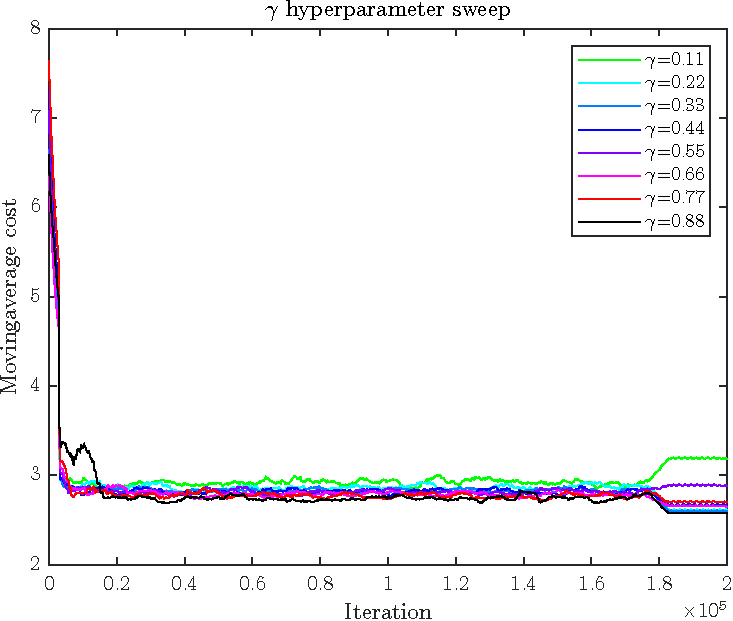
\includegraphics[width=1\linewidth]{figures/GammaSweepTabRealH.pdf}
		\caption{Gamma sweep full plot.}
		\label{fig:GammaSweepTabularFull}
	\end{subfigure}%
	\begin{subfigure}{.5\textwidth}
		\centering
		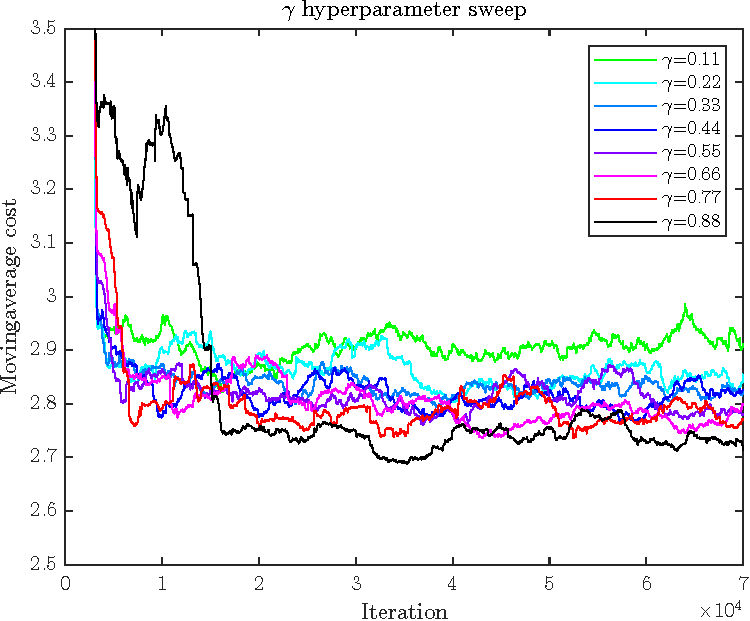
\includegraphics[width=1\linewidth]{figures/GammaSweepTabRealHZoom.pdf}
		\caption{Initial convergence.}
		\label{fig:GammaSweepTabularZoom}
	\end{subfigure}
	\caption{Gamma sweep showing the full plot (a), and a zoom focused on initial convergence (b).}
	\label{fig:Gammasweep}
\end{figure}

\cref{fig:Gammasweep} shows gamma sweep. There is also one clear tendency here, higher values converge slower, but settles lower once they have converged. The final moving average convergence value after the cutoff of all  $\gamma$ values fall within the margin of randomness, and therefore this area receives no further consideration.

\begin{figure}[h!]
	\centering
	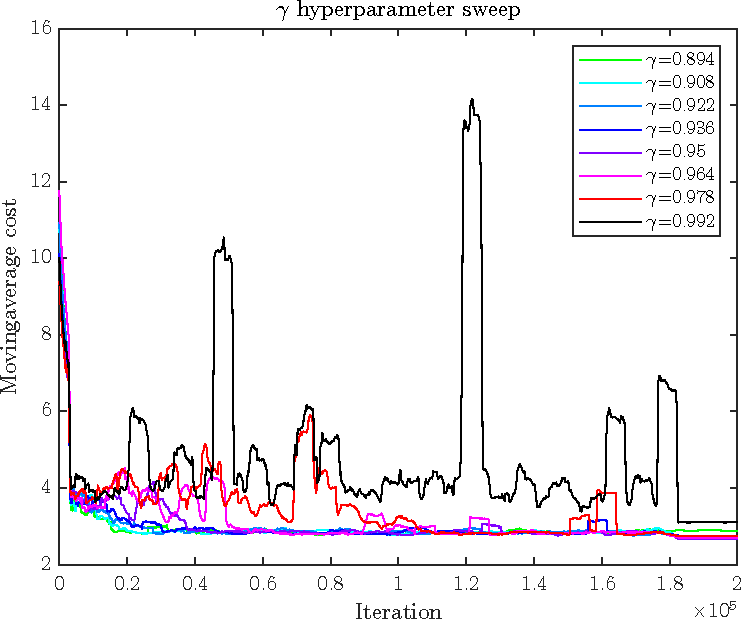
\includegraphics[width=0.7\linewidth]{figures/GammaSweepTabRealHNarrow.pdf}
	\caption{Additional narrow gamma sweep, including a finer sweep of high gamma values.}
	\label{fig:GammaSweepTabularNarrow}
\end{figure} 

\cref{fig:GammaSweepTabularNarrow} shows a narrow sweep of the very high values. A narrow sweep is performed for high values because the best value was expected to be in this range. Sweeps on previous iterations of the simulations scripts showed good performance with high $\gamma$, however, this is no longer valid. Higher values clearly slow convergence even further, to the point of not converging at all. Final convergence does not improve.
We choose a value of 0.77, since it is desired to converge as low as possible as fast as possible. Therefore we choose the highest values that does not increase convergence time a lot.

\begin{figure}[h!]
	\centering
	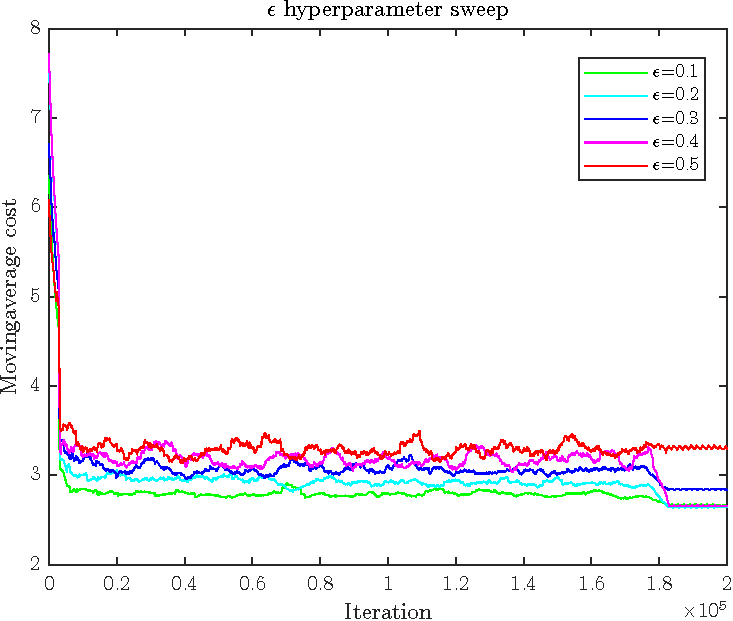
\includegraphics[width=0.7\linewidth]{figures/EpsilonSweepTabRealHWide.pdf}
	\caption{Epsilon sweep of relevant values between 0.1 and 0.5.}
	\label{fig:EpsilonSweepTabular}
\end{figure} 


\cref{fig:EpsilonSweepTabular} shows epsilon sweep for relevant values of $\epsilon$ ranging from 0.1 to 0.5, higher values means we are more random than not. A small $\epsilon$ standout as both yielding the smallest training cost, and lowest final convergence. This is expected from previous sweeps. Higher epsilon means the random influence leading up to the cutoff is greater\footnote{Remember we choose a quite high $\alpha = 0.9$.}, resulting in a greater spread of final convergence. Note $\epsilon = 0.1,0.4$ converge to similar final cost, showing that the high epsilon only increases the spread, not necessarily resulting in worse performance. The higher training cost is an obvious result of more random actions. We choose $\epsilon = 0.1$.

Final parameters are:
\begin{equation*}
	\alpha = 0.9 \hspace{1cm} \gamma = 0.77 \hspace{1cm} \epsilon = 0.1
\end{equation*}

  
\begin{figure}[h!]
	\centering
	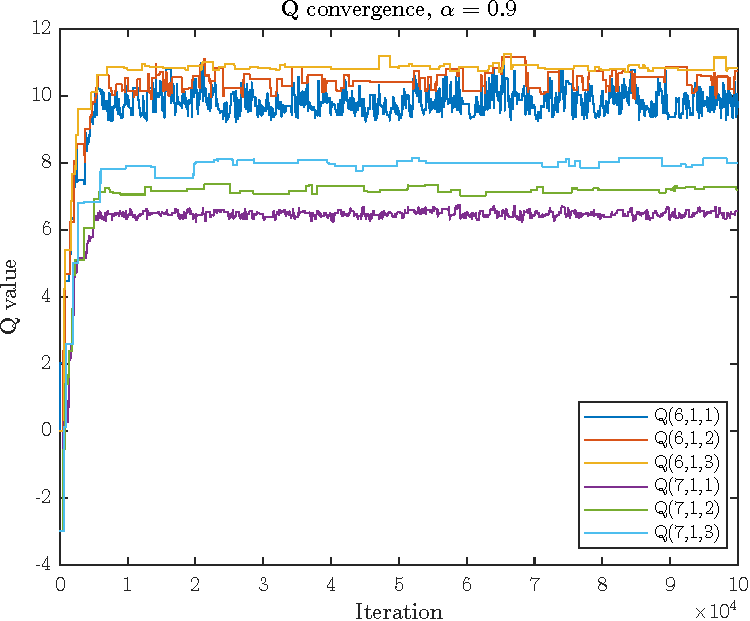
\includegraphics[width=0.7\linewidth]{figures/QConvergence09.pdf}
	\caption{Q convergence. Values for two different heights are shown, the lower height $h=7$, has an offset to add visual clarity to the plot.}
	\label{fig:Qconvergence09}
\end{figure} 

\begin{figure}[h!]
	\centering
	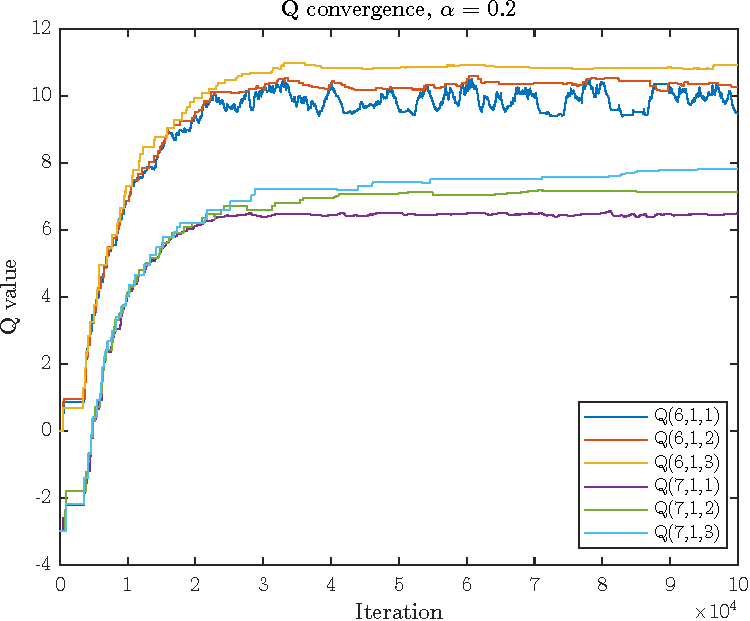
\includegraphics[width=0.7\linewidth]{figures/QConvergence02.pdf}
	\caption{Q convergence for reduced $\alpha$. Offset for visual clarity included again.}
	\label{fig:Qconvergence02}
\end{figure} 

As a few final remarks, we consider the convergence of the Q values, and with it an extra parameter evaluation on $\alpha = 0.2$ and $\alpha = 0.9$. The extra evaluation is included to present different water level behaviour, as seen in this paragraph. Q value convergence is a candidate for an alternative evaluation scheme instead of moving average cost for sweeps. \cref{fig:Qconvergence09} and \cref{fig:Qconvergence02} show Q convergence for $\alpha = 0,9$ and $\alpha = 0.2$ respectively. Notice that the \textit{chaoticness} of each signal is an indication of how often that specific state-action combination appears. Obviously the higher $\alpha$ value results in more oscillations, a lower value was included for comparison. Additionally, \cref{fig:QConvergenceBehavior} shows 5 simulations of reservoir water level plotted in the same plot. Here we see the impact of oscillations from high $\alpha$ are minor, the variance of the convergence of $\alpha = 0.2$ is smaller, but with more and greater outliers. Both share the same mean.

These results are more related to specific systems, and \textit{good} behaviour for that system. Sometimes less water level variance could be desired over fast convergence, therefore choosing a lower $\alpha$.

\begin{figure}
	\centering
	\begin{subfigure}{.5\textwidth}
		\centering
		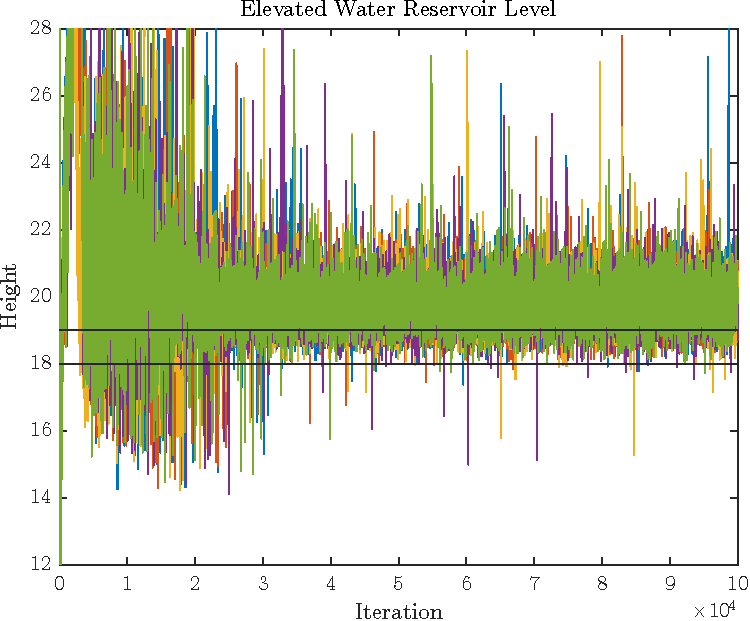
\includegraphics[width=1\linewidth]{figures/ConvergenceHeight02.pdf}
		\caption{5 simulations using $\alpha = 0.2$}
		\label{fig:5sims1}
	\end{subfigure}%
	\begin{subfigure}{.5\textwidth}
		\centering
		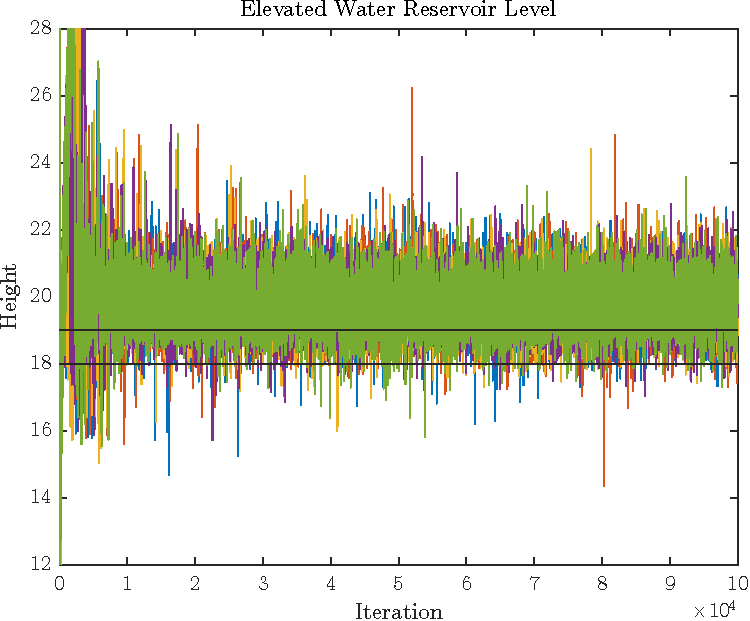
\includegraphics[width=1\linewidth]{figures/ConvergenceHeight09.pdf}
		\caption{5 simulations using $\alpha = 0.9$}
		\label{fig:5sims2}
	\end{subfigure}
	\caption{5 simulations in each plot used for comparison of high and low alpha, and the resulting behaviour of reservoir water level. Black lines are inserted at heights 18 and 19, to make differences more visible. Each colour is 1 of the 5 simulations.}
	\label{fig:QConvergenceBehavior}
\end{figure}

\newpage \clearpage

\subsection{Tabular Results}
Here we show simulation results using the swept parameters.

\begin{figure}[h!]
	\centering
	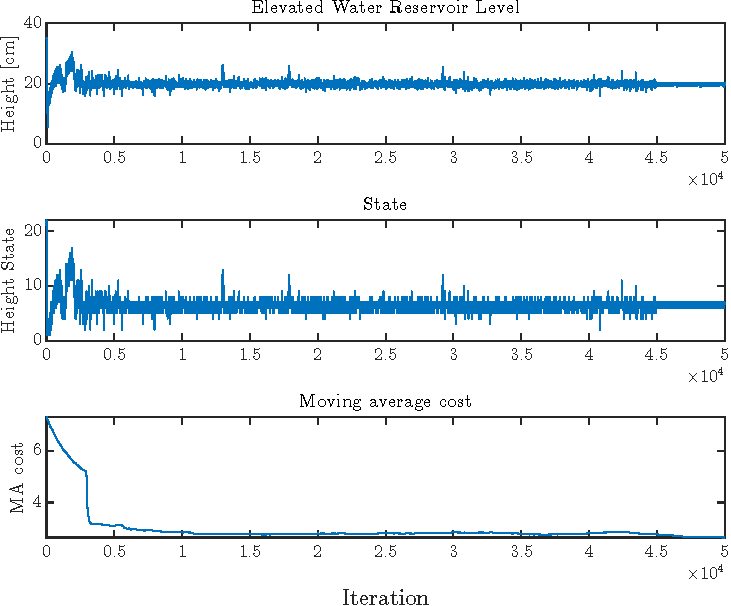
\includegraphics[width=0.7\linewidth]{figures/TabularResults2.pdf}
	\caption{Tabular Q learning results, showing elevated water reservoir level, state and moving average cost.}
	\label{fig:Tabularresults1}
\end{figure} 

\cref{fig:Tabularresults1} show reservoir water level, height state and the moving average cost. Water level converge nicely around the barrier at 20\si{cm}. The states are clearly explored from the bottom first, due to Matlab always choosing the first option when results of the \textit{minimum function} are equal, resulting in descending behaviour when initialising at 0. Let the term \textit{turnaround} denote to the ability to stop ascending-exploration of the height state, and begin to descend toward optimal values, before exploring the entire height space. This happens at iteration 1800 in \cref{fig:ResultRightZoom}. The \textit{turnaround} is unexpected, but results in much faster convergence as many states are unexplored. Some theories of why this happens is discussed in \cref{chap:Discussion}.

\begin{figure}[h!]
	\centering
	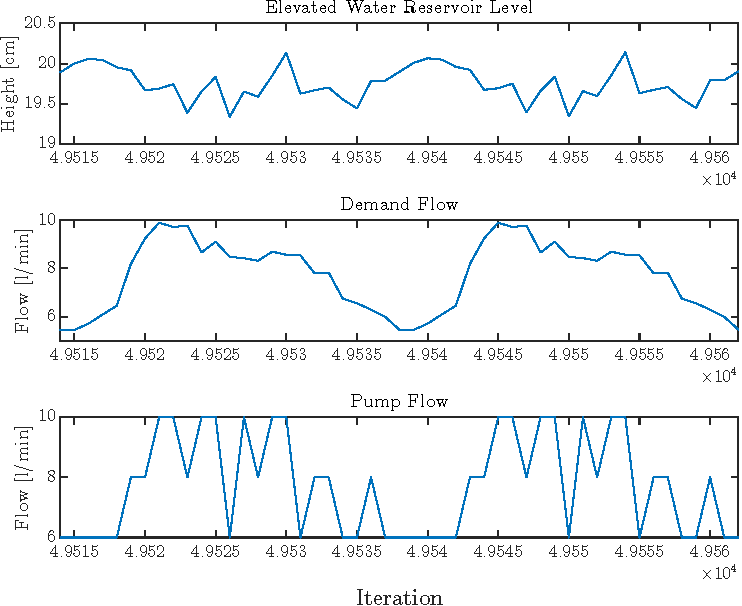
\includegraphics[width=0.7\linewidth]{figures/TabularResults1.pdf}
	\caption{48 hours tabular results,taken after the cutoff. Shows relationship between height, demand- and pump flow.}
	\label{fig:TabularResults2}
\end{figure} 

\cref{fig:TabularResults2} shows a 48 hour period after the cutoff. This clearly shows the dynamics between demand flow and pump flow (actions).

\begin{figure}
	\centering
	\begin{subfigure}{.5\textwidth}
		\centering
		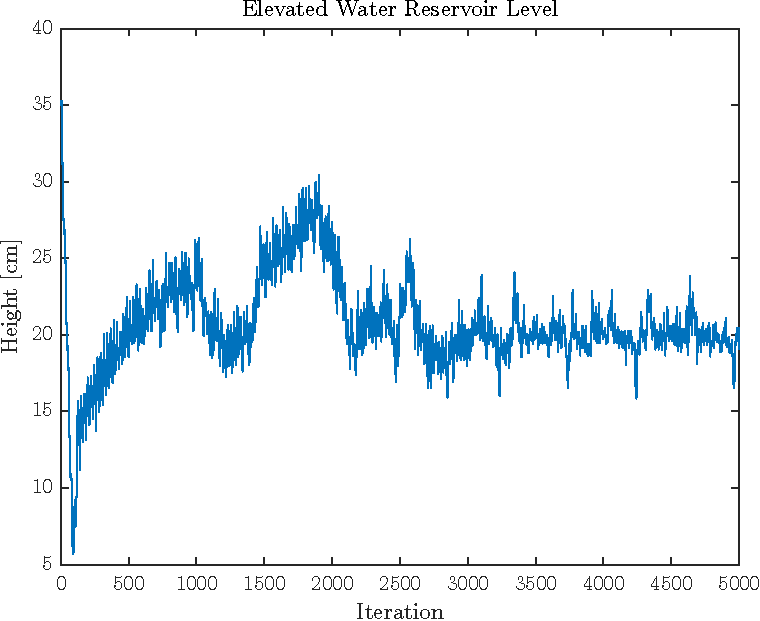
\includegraphics[width=1\linewidth]{figures/TabularResults3.pdf}
		\caption{Initial convergence.}
		\label{fig:ResultRightZoom}
	\end{subfigure}%
	\begin{subfigure}{.5\textwidth}
		\centering
		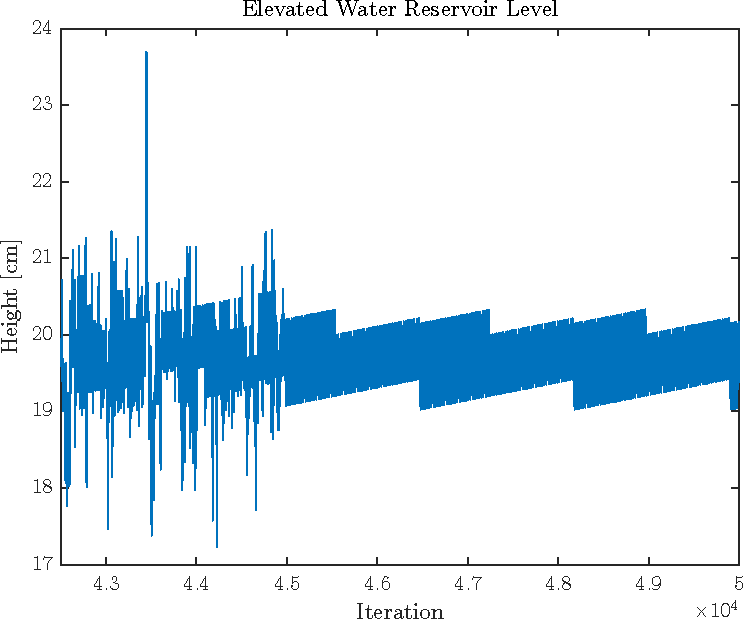
\includegraphics[width=1\linewidth]{figures/TabularResults4.pdf}
		\caption{Cutoff convergence.}
		\label{fig:ResultLeftZoom}
	\end{subfigure}
	\caption{Elevated water reservoir level results focused on initial convergence (a), and cutoff convergence (b).}
	\label{fig:ResultZoom}
\end{figure}

\cref{fig:ResultZoom} shows a zoomed image of the reservoir water level in the beginning and end of the simulation. In \cref{fig:ResultRightZoom}, notice the fast descend in the beginning (iteration 100), this is because action 1 is always chosen. Q is initialised to 0 for all state action pairs, and Matlab's min function always selects the first entry when min evaluations are equal. The rapid ascend back to 15, is because the state never changes, all states below 15 are set to state 1 due to height discretisation. Above the height of 15, dynamics slow down as new states are encountered at every height. 

The zigzag pattern in \cref{fig:ResultLeftZoom} is a result of slightly scewed demand balancing. The optimal policy simply results in a slight amount of excess water for every 24 hour period. If pumps or demand is altered slightly a smooth non-zigzag result can be obtained.

\clearpage \newpage

\section{Continuous Height, and Discrete Time and Action Q-Learning}\label{sec:sim1D}

As explained in \cref{sec:WDN1D} the action-value function can be approximated as:

\begin{equation}
	\hat{Q}\bigg(h(k),\textbf{w}_{t(k),a(k)}\bigg) =  \textbf{w}_{t(k),a(k)}\textbf{x}\bigg(h(k)\bigg)
\end{equation}

This section present simulation results obtained when applying continuous height, and discrete time and action Q-learning, to the water distribution in \cref{chap:WDN}. 

Weight vector is initialised to zero and updated according to \cref{alg:FuncApproxQ-learning} and radial basis functions are placed as explained in \cref{sec:WDNFunctionApproximationQ-Learning}. Hyper-parameter sweep is done similarly as in \cref{sec:TabularHSweep}, but plots are not shown, because tendencies cannot be seen in a single plot. Instead many simulations are done with varying combinations of hyper parameters, to build an intuition about system behaviour. The chosen parameters are:

\begin{equation*}
	\alpha = 0.4 \hspace{1cm} \gamma = 0.95 \hspace{1cm} \epsilon = 0.1
\end{equation*}

\begin{figure}[h!]
	\centering
	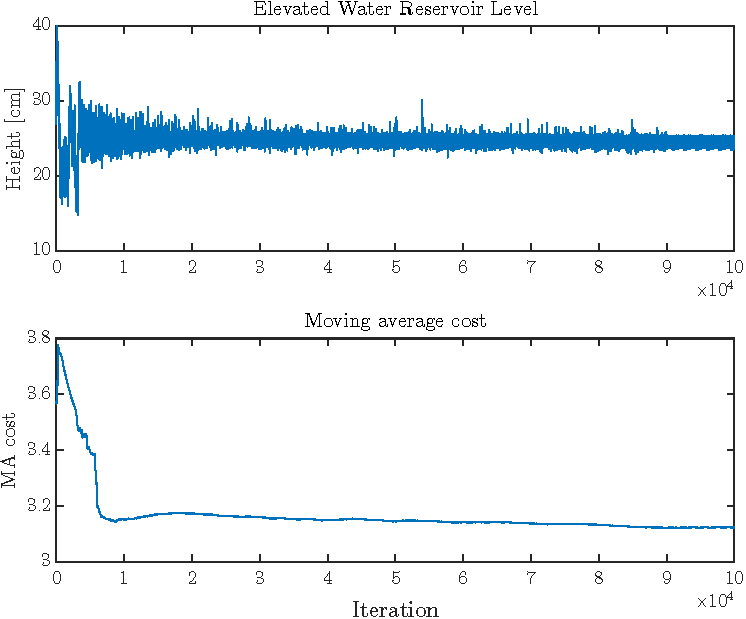
\includegraphics[width=0.7\linewidth]{figures/ContiniousHResults2.pdf}
	\caption{Continuous height approximation Q learning results. Showing elevated water reservoir level and moving average cost.}
	\label{fig:ContiniousHResults1}
\end{figure}

\cref{fig:ContiniousHResults1} presents water level in the elevated water reservoir and moving average of the cost function. Most noticeable is the tendency to settle much higher than the lower barrier, this is discussed further in \cref{chap:Discussion}. The benefit of generalisation is very apparent as the algorithm does not have to explore as aggressively to find the optimal policy.

\begin{figure}[h!]
	\centering
	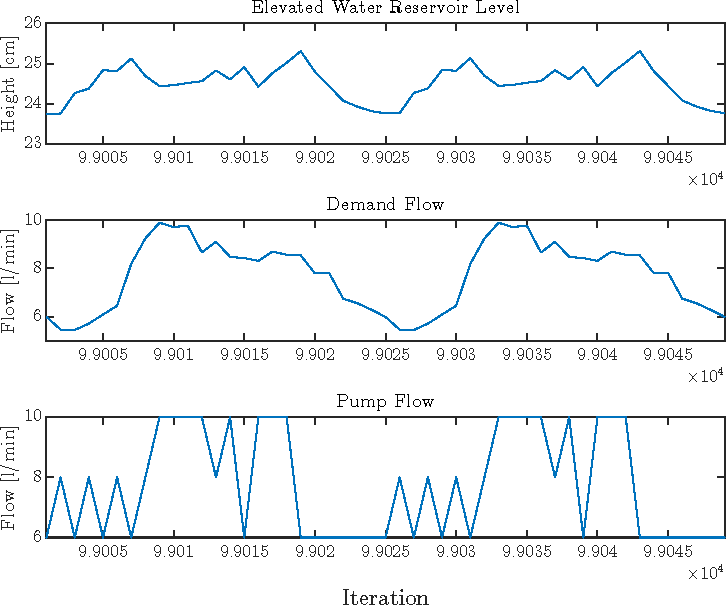
\includegraphics[width=0.7\linewidth]{figures/ContiniousHResults1.pdf}
	\caption{48 hours continuous height results, taken after cutoff. Shows relationship between height, demand- and pump flow.}
	\label{fig:ContiniousHResults2}
\end{figure} 

\cref{fig:ContiniousHResults2} shows a 48 hour period after the cutoff. It shows water levels similar to tabular method, pump flow (actions) are also similar, but clearly not the same. Although action value functions are obviously not exactly the same for both methods, this shows some proof of the concept that there exists several optimal policies (pump flows) which yield the same value function. 

\clearpage \newpage
\begin{figure}[h!]
	\centering
	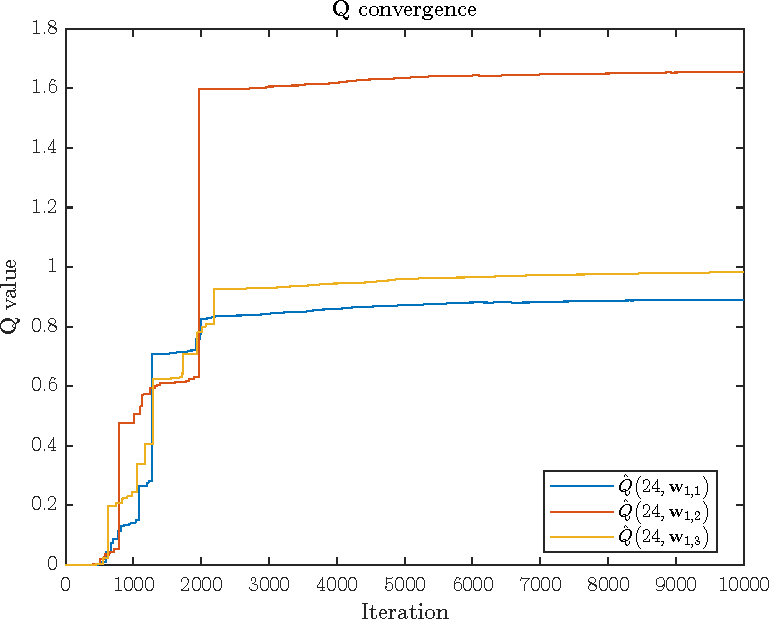
\includegraphics[width=0.7\linewidth]{figures/ContiniousHResults3.pdf}
	\caption{Q convergence for continuous height, at $h = 24,$ $t = 1$.}
	\label{fig:ContiniousHeightQConvergence}
\end{figure}
 
\cref{fig:ContiniousHeightQConvergence} presents convergence of approximated action value for height $ h=24\si{cm} $ and time $ t=1 $. Notice the x-axis is zoomed on iterations $0 - 10000$ to show the initial convergence. We can see the impact of generalisation by noticing that in the beginning (iteration 0 - 2000) of \cref{fig:ContiniousHResults1} the height is explored around $h=20$, however, \cref{fig:ContiniousHeightQConvergence} showing the Q value at $h=24$ shows changes at these iterations.


%Here we see some large jumps, even though the water level in the tank does not equal 24 at that time. These jumps happen when at $t = 1$ the specific action is made at some other water level. Due to generalisation, if that action yield a high cost, likely because the barrier is hit, there will be a large jump for all nearby heights.

\newpage

\iffalse
\subsection{Hyperparameters}
There are several hyperparameters which must be chosen, here we perform sweeps and evaluate performance to find a suitable hyperparameter value. Initial values are arbitrarily chosen, and each hyperparameter is then sequentially sweept. Initial values are shown below, parameters appear in the order they are swept:

\begin{equation*}
	\alpha = 0.1 \hspace{1cm} \gamma = 0.9 \hspace{1cm} \epsilon = 0.1
\end{equation*}

Sweeps are performed over singular parameters, ideally combinations of all parameters should be sweept, but we deem this too resource demanding. Performance is evaluated by looking at a moving average of the cost with a large window size, which helps smoothing out randomness. The final 10$\%$ of all simulations are without learning ($\alpha = 0$) or randomness ($\epsilon = 0$), this gives a more explicit indication of performance\footnote{E.g a large epsilon results in higher cost while learning, but lower cost after learning}. 

\begin{figure}[h!]
	\centering
	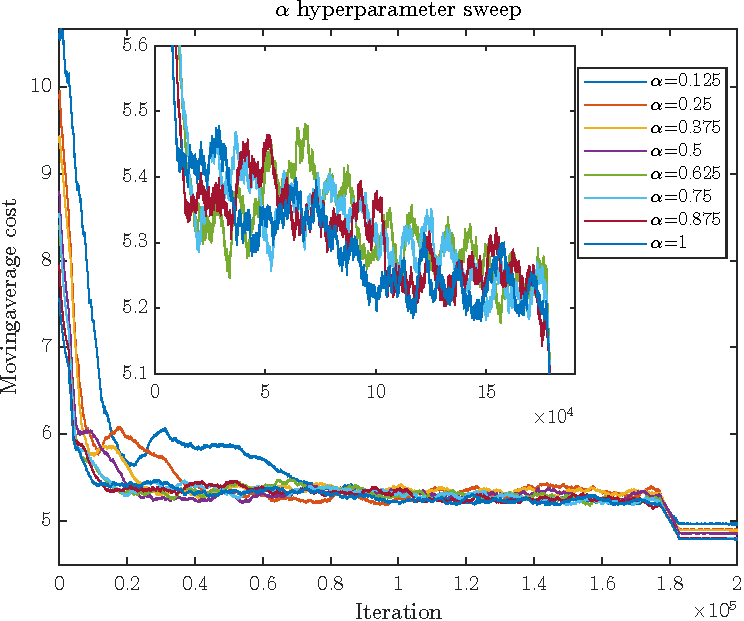
\includegraphics[width=0.7\linewidth]{figures/AlphaSweepApproxBest.pdf}
	\caption{Alpha sweep. Insert shows a zoomed image of the four largest alpha values.}
	\label{fig:AlphaSweep}
\end{figure} 

\cref{fig:AlphaSweep} shows different alpha values. Two tendencies are clear, larger alpha values both converge faster and to a lower cost. The insert shows a zoomed image of the four greatest alpha values. Here there are no clear discrephancies, and differences fall within the margin of randomness.

Simulations with $\alpha > 1$ shows cost diverging, although for $\alpha < 1.1$ cost sometimes converge as above. This correlate well with the properties in \cref{eq:alphaAssumptions}. We choose to use $\alpha = 0.75$ as this gives similar performance to higher values, and we assume higher values can cause problems if more weights are introduced.

\newpage
\clearpage

\begin{figure}[h!]
	\centering
	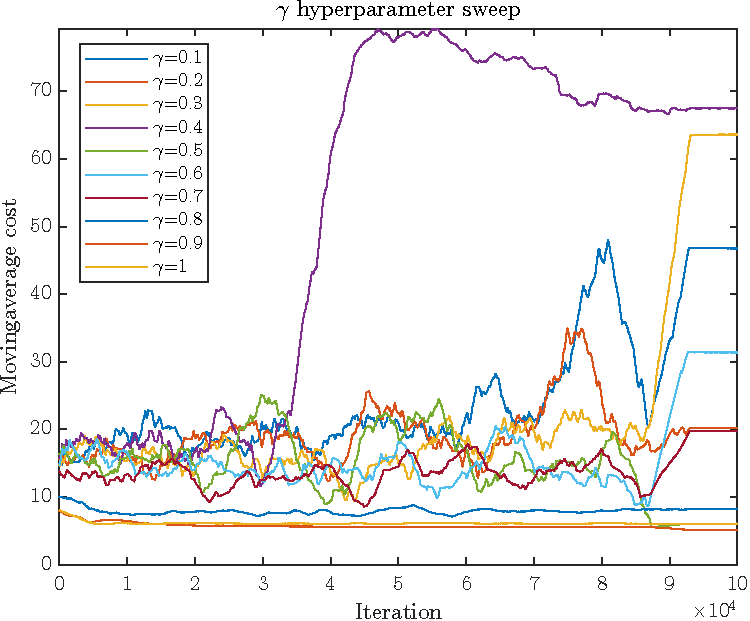
\includegraphics[width=0.7\linewidth]{figures/GammaSweepApproxWide.pdf}
	\caption{Wide gamma sweep. This is the first gamma sweep, sweeping over a wide range of values.}
	\label{fig:WideGammaSweep}
\end{figure} 

\cref{fig:WideGammaSweep} shows the first of two gamma sweeps. This is a wide sweep, considering a large range of values, this is done to identify where a narrow sweep should be performed. It is obvious that very high values yield best performance.

\begin{figure}[h!]
	\centering
	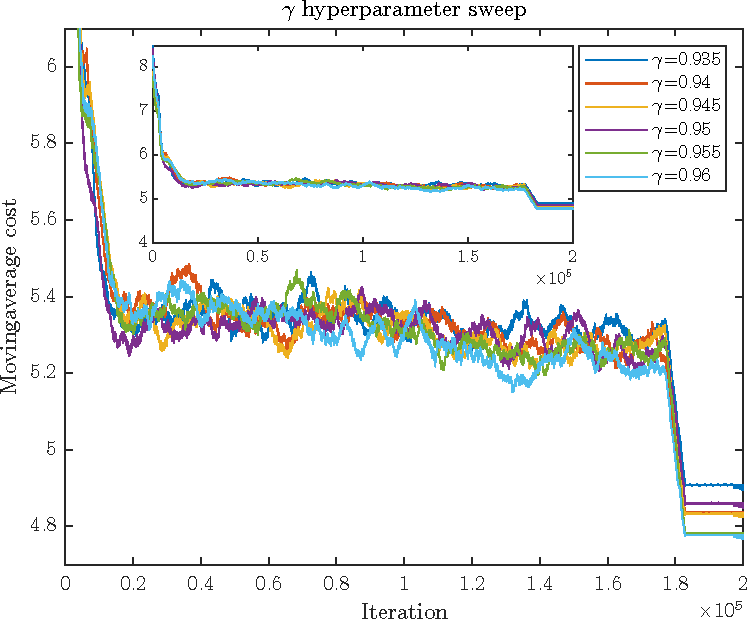
\includegraphics[width=0.7\linewidth]{figures/GammaSweepApproxNarrow.pdf}
	\caption{Narrow gamma sweep.}
	\label{fig:NarrowGammaSweep}
\end{figure} 

\cref{fig:NarrowGammaSweep} shows a narrow sweep at high values. Differences are susceptible to randomness, therefore multiple simulations of the above figure was performed, showing higher values consistently converge to a lower cost. \textit{We will see if even higher values are better, this plot lacks even higher values}.


\newpage
\clearpage
\begin{figure}[h!]
	\centering
	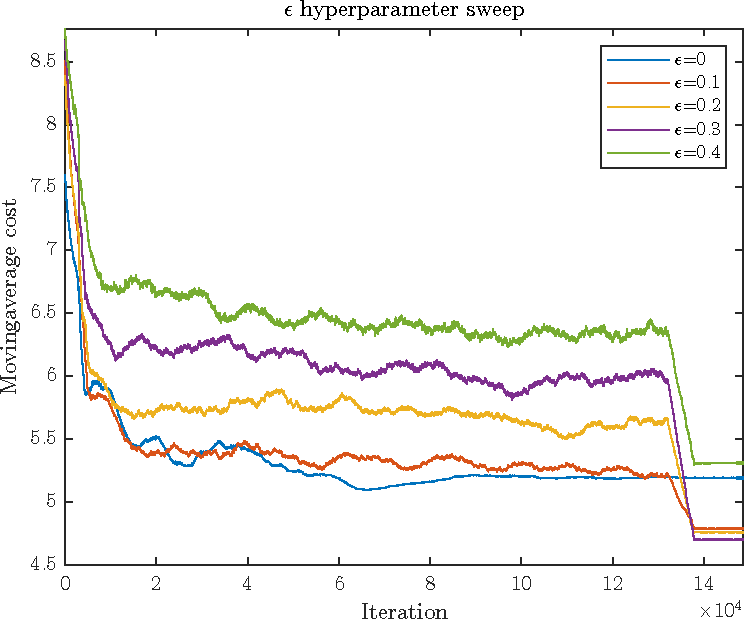
\includegraphics[width=0.7\linewidth]{figures/EpsilonSweepApprox.pdf}
	\caption{Epsilon sweep.}
	\label{fig:EpsilonSweep}
\end{figure} 

\cref{fig:EpsilonSweep} shows epsilon in the meaningful range between $0 < \epsilon < 0.5$, $\epsilon = 0$ is included for reference. At first glance the greedy algorithm without randomness looks decent, however, adding randomness leads to a lower convergence. More randomness seems to yield lower convergence up to a threshold. The highest epsilon (green), is worse than no randomness (blue), likely because the randomness explores actions in parts of the state space that are far from the optimal policy. There is simply not enough greediness to keep the algorithm in the area of the state space which contain the optimal policy, leading to pointless exploration.

A high epsilon leads to better performance after training, but at the sacrifice of performance while training, clearly shown by the layers in the figure. Therefore we choose $epsilon = 0.1$ to have the best performance while training, and still get the lower convergence that comes with exploration.
\fi


\clearpage
\newpage
\section{Continuous Level and Time, Discrete Action Q-Learning}


As explained in \cref{sec:WDN2D} The action value can be estimated using function approximation in both the height and time:

\begin{equation}
	\hat{Q}\bigg(h(k),t(k),\textbf{w}_{a(k)}\bigg) =  \textbf{w}_{a(k)}\textbf{x}\bigg(h(k),t(k)\bigg)
\end{equation}

Height approximation is done using weights and centers as previously. And time is approximated as presented in \cref{sec:WDN2D}. The weight vector is initialised and updated according to \cref{alg:ContFuncApproxQ-learning}. As previously, hyper parameter are swept but not shown. The following parameters are used:

\begin{equation*}
	\alpha = 0.2 \hspace{1cm} \gamma = 0.95 \hspace{1cm} \epsilon = 0
\end{equation*}

Notice $\epsilon = 0$, it was found that any randomness causes worse performance, and it is therefore not used. We present thought on \textit{implicit exploration} caused by Q initialisation and oscillating demand in \cref{chap:Discussion}.

\begin{figure}[h!]
	\centering
	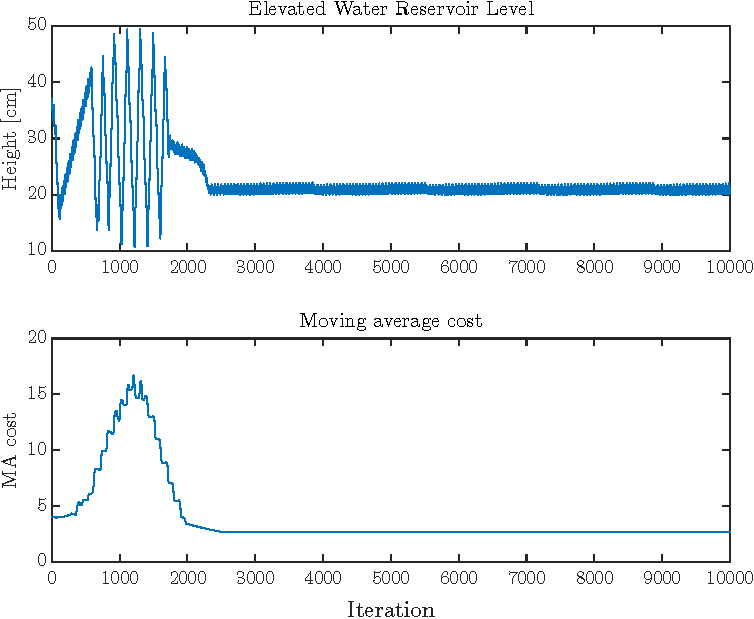
\includegraphics[width=0.7\linewidth]{figures/DoubleContResults1.pdf}
	\caption{Continuous height and time approximation Q learning results. Showing elevated water reservoir level and moving average cost.}
	\label{fig:DoubleContResults1}
\end{figure} 

\cref{fig:DoubleContResults1} presents water level in the elevated water reservoir and moving average of the cost function. Here we see a very defined initial learning, before converging to a final convergence value almost immediately. Notice that the final convergence is smoother than usual since $\epsilon = 0$. The first \textit{linear} learning explores the same state space as height approximation method, but then explores much broader. A very fast convergence around iteration 2200 is achieved, showing the power of generalisation. The final convergence value is also similar to that of the tabular method (better than height approximation). Notice the tendency to converge higher than the optimal value around $h_\star \approx 20$, which also was visible for height approximation, almost appears around iteration  2000. This tendency is even more apparent for different $\alpha$ values.

\begin{figure}[h!]
	\centering
	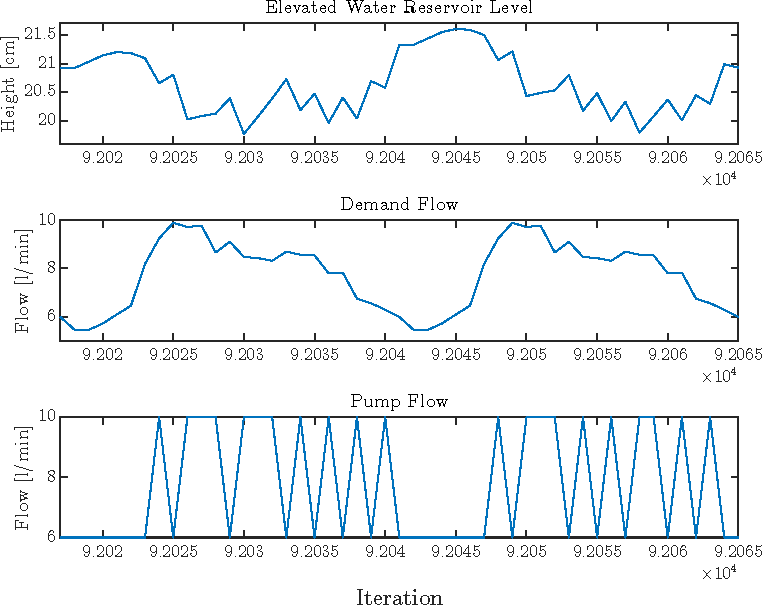
\includegraphics[width=0.7\linewidth]{figures/DoubleContResults2.pdf}
	\caption{48 hours continuous height and time results, taken after cutoff. Shows relationship between height, demand- and pump flow.}
	\label{fig:DoubleContResults2}
\end{figure} 

\cref{fig:DoubleContResults2} shows the same comparison as for the other methods. Notice there is no cutoff since this simulation does not include randomness. This means the pump profile is different for each 24 hour period, this tendency is also apparent if the cutoff is included, which would usually force equal action profiles for each 24 hour period. It seems generalising on time gives the algorithm more freedom, we do not grasp the full context to this \textit{feature}.

\begin{figure}
	\centering
	\begin{subfigure}{.5\textwidth}
		\centering
		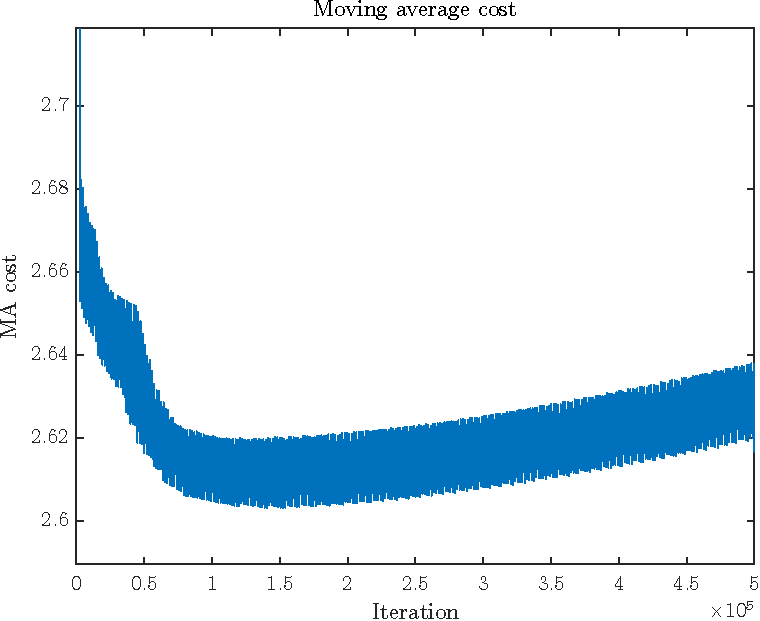
\includegraphics[width=1\linewidth]{figures/DoubleApprox02.pdf}
		\caption{Divergence of $\alpha = 0.2$.}
		\label{fig:Divergence02}
	\end{subfigure}%
	\begin{subfigure}{.5\textwidth}
		\centering
		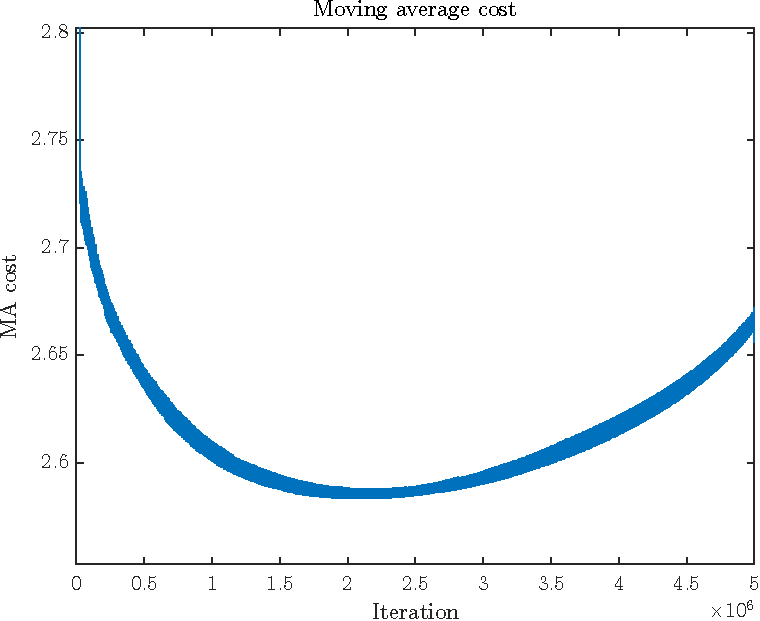
\includegraphics[width=1\linewidth]{figures/DoubleApprox001.pdf}
		\caption{Divergence of $\alpha = 0.01$.}
		\label{fig:Divergence001}
	\end{subfigure}
	\caption{Comparison of moving average cost beteween $\alpha = 0.2, \hspace{0.2cm} 0.01$.}
	\label{fig:DivergenceComparison}
\end{figure}

Although this method converges very fast, an issue is found if the simulation is extended. \cref{fig:DivergenceComparison} shows moving average costs for long simulations using $\alpha = 0.2\ \text{and}\ \alpha = 0.01$, both clearly diverge. We suspect this is caused by \textit{deadly triad} \cite{Sutton2020}. The deadly triad describes the danger of instability and divergence when combining the three following element: Function approximation, bootstrapping and off-policy training (Q-learning). On policy learning like \textit{SARSA} could be used to circumvent this issue.


\section{Method Comparison}

Function approximation has shown to be a very powerful tool, but also dangerous. Complexity increases drastically when approximating, intuition and knowledge about the algorithm's behaviour is much harder to obtain. We will make this comparison from the perspective of lab and real world implementation. In this context, double approximation is too parameter sensitive and likely to diverge, to be considered for real world implementation. The tabular method, showing similar convergence as height approximation, and even better final convergence, requires operation dangerously close to the  bottom of the tank. Height approximation show good performance and does not need to explore dangerous areas, therefore this method is the most suited for implementation at this stage of development. The performance of this method is further tested as it is applied to our water distribution network test setup in the following chapter.